\documentclass{standalone}
\usepackage[compat=1.1.0]{tikz-feynman}
\begin{document}
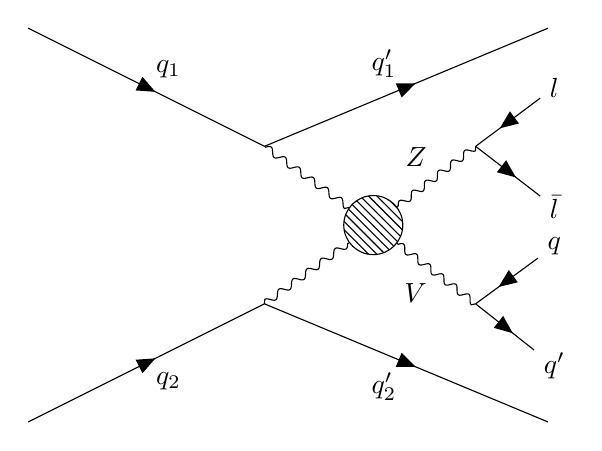
\begin{tikzpicture}
    \begin{feynman}
        \vertex (q1);
        \vertex [right=3cm of q1] (a0);
        \vertex [below=1.5cm of a0] (a);
        \vertex [right=3.6cm of a] (t01);
        \vertex [above=1.5cm of t01] (t1);
        \vertex [below=1cm of a] (b0);
        \vertex [blob, right=1cm of b0] (b) {};
        \vertex [right=1.3cm of b] (f01);
        \vertex [above=1cm of f01] (f1);
        \vertex [right=1cm of f1] (f001);
        \vertex [above=0.5cm of f001] (f2) {\(l\)};
        \vertex [below=0.5cm of f001] (f3) {\(\bar{l}\)};
        \vertex [right=1.3cm of b] (f04);
        \vertex [below=1cm of f04] (f4);
        \vertex [right=1cm of f4] (f004);
        \vertex [above=0.5cm of f004] (f5) {\(q\)};
        \vertex [below=0.5cm of f004] (f6) {\(q'\)};
        \vertex [below=1cm of b0] (c);
        \vertex [left=3cm of c] (q02);
        \vertex [below=1.5cm of q02] (q2);
        \vertex [right=3.6cm of c] (t02);
        \vertex [below=1.5cm of t02] (t2);
        \diagram* {
        (q1) -- [fermion, edge label=\(q_{1}\)] (a) -- [fermion, edge label=\(q'_{1}\)] (t1),
        (a) -- [boson] (b) -- [boson] (c),
        (q2) -- [fermion, edge label'=\(q_{2}\)] (c) -- [fermion, edge label'=\(q'_{2}\)] (t2),
        (b) -- [boson, edge label=\(Z\)] (f1),
        (b) -- [boson, edge label'=\(V\)] (f4),
        (f2) -- [fermion] (f1) -- [fermion] (f3),
        (f5) -- [fermion] (f4) -- [fermion] (f6),
        };
    \end{feynman}
\end{tikzpicture}
\end{document}